\documentclass[11pt]{article}

\usepackage{fullpage,fourier,amsmath,amssymb}
\usepackage{listings,color,url}
\usepackage{mdframed}
\usepackage{epigraph}
\usepackage[x11names]{xcolor}
\usepackage{gensymb}
\usepackage{forest}
\usepackage{float}
\usepackage{tikz}
\usetikzlibrary{arrows}
\usepackage[colorlinks=true,urlcolor=blue]{hyperref}
\usetikzlibrary{positioning,matrix}

\title{Assignment 3 \\ Sorting: Putting your affairs in order}
\author{Prof. Darrell Long \\ CSE 13S -- Winter 2023}
\date{Due: February 5$^\text{th}$ at 11:59\,pm}

\usepackage{fancyhdr}
\pagestyle{fancy}
\fancyhf{}

\fancypagestyle{plain}{%
  \fancyhf{}
  \renewcommand{\headrulewidth}{0pt}
  \renewcommand{\footrulewidth}{0pt}
  \lfoot{\textcopyright{} 2021 Darrell Long}
  \rfoot{\thepage}
}

\pagestyle{plain}

\definecolor{codegreen}{rgb}{0,0.5,0}
\definecolor{codegray}{rgb}{0.5,0.5,0.5}
\definecolor{codepurple}{rgb}{0.58,0,0.82}

\lstloadlanguages{C,make,python,fortran,bash}

\lstdefinestyle{bashstyle}{
  language=bash,
  basicstyle=\small\ttfamily,
  numbers=none,
  frame=tb,
  columns=fullflexible,
  backgroundcolor=\color{yellow!10},
  linewidth=0.9\linewidth,
  xleftmargin=0.1\linewidth,
  aboveskip=1.25em,
  belowskip=1.25em,
  breakatwhitespace=false,
  breaklines=true,
  showstringspaces=false,
  keepspaces=true,
  showspaces=false,
  showtabs=false,
  tabsize=4
}

\lstdefinestyle{plainstyle}{
  keywords={},
  stringstyle=\color{black},
  basicstyle=\small\ttfamily,
  numbers=none,
  frame=tb,
  columns=fullflexible,
  backgroundcolor=\color{yellow!10},
  linewidth=0.9\linewidth,
  xleftmargin=0.1\linewidth,
  aboveskip=1.25em,
  belowskip=1.25em,
  breakatwhitespace=false,
  breaklines=true,
  showstringspaces=false,
  keepspaces=true,
  showspaces=false,
  showtabs=false,
  tabsize=4
}

\lstdefinestyle{c99}{
    language=C,
    morekeywords={
      bool, uint8_t, uint16_t, uint32_t, uint64_t,
      int8_t, int16_t, int32_t, int64_t
    },
    upquote=true,
    commentstyle=\color{codegreen},
    keywordstyle=\color{magenta},
    identifierstyle=\color{black},
    stringstyle=\color{codepurple},
    basicstyle=\ttfamily,
    breakatwhitespace=false,
    breaklines=true,
    captionpos=b,
    keepspaces=true,
    showspaces=false,
    showstringspaces=false,
    showtabs=false,
    numbers=left,
    numbersep=7pt,
    numberstyle=\ttfamily\color{black!25},
    xleftmargin=12pt,
    tabsize=4
}

\lstdefinestyle{python}{
    language=python,
    upquote=true,
    commentstyle=\color{codegreen},
    keywordstyle=\color{magenta},
    identifierstyle=\color{black},
    stringstyle=\color{codepurple},
    basicstyle=\ttfamily,
    breakatwhitespace=false,
    breaklines=true,
    captionpos=b,
    keepspaces=true,
    showspaces=false,
    showstringspaces=false,
    showtabs=false,
    numbers=left,
    numbersep=7pt,
    numberstyle=\ttfamily\color{black!25},
    xleftmargin=12pt,
    tabsize=4
}

\usepackage[most]{tcolorbox}

\newtcolorbox{prelab}[1]{
  colback=red!5!white, colframe=red!75!black, title=#1
}

\newtcblisting{codelisting}[2][]{
  title=#2, #1,
  fonttitle=\bfseries,
  colframe=black!80,
  listing only,
  listing options={basicstyle=\ttfamily,style=c99},
  top=-5pt,
  bottom=-5pt,
  enlarge top by=10pt
}

\newtcblisting{pythonlisting}[2][]{
  title=#2, #1,
  fonttitle=\bfseries,
  colframe=black!80,
  listing only,
  listing options={basicstyle=\ttfamily,style=python},
  top=-5pt,
  bottom=-5pt,
  enlarge top by=5pt
}

\newcommand\Warning{%
 \makebox[1.4em][c]{%
 \makebox[0pt][c]{\raisebox{.1em}{\small!}}%
 \makebox[0pt][c]{\color{red}\Large$\bigtriangleup$}}}%

\newenvironment{funcdoc}[1]{\subsubsection*{\underline{\textbf{\texttt{#1}}}}}{}

\newcommand{\monkey}[1]{
  \begin{center}
    \includegraphics[width=0.35\textwidth]{../monkey.jpg} \\
    \emph{#1}
  \end{center}
}


\begin{document}

\maketitle

\section{Introduction}

\lettrine[lines=3]{I}{n number theory}, a perfect number is a
positive integer that is equal to the sum of its positive divisors,
excluding the number itself (called its \emph{proper divisors}). For instance, $6$ has divisors $1, 2$ and
$3$ (excluding itself), and $1 + 2 + 3 = 6$, so $6$ is a perfect number.

The sum of divisors of a number, excluding the number itself, is
called its \emph{aliquot sum}, $s (n)$ of a positive integer $n>0$
is the sum of all \emph{proper divisors} of $n$, that is, all
divisors of $n$ other than $n$ itself.  When we write $d\mid n$ we mean
that $n \div d$ is an integer with no remainder, and when we write
$d \nmid n$ then $n \div d$ has a remainder.  So we define $s(n)$ as,
$$s (n)=\sum\nolimits_{d\mid n,\ 0<d < n}d.$$
A perfect number is one that is equal to its aliquot sum. Equivalently, a perfect number
is a number that is half the sum of all of its positive divisors including itself; in symbols,
$\sigma_1 (n) = 2 n$ where $\sigma_1$
is the sum-of-divisors function.
That is,
$$\sigma_1 (n)=\sum\nolimits_{d\mid n,\ 0<d\le n}d.$$
For instance, $28$ is perfect as
$\sigma_1(28) = 1 + 2 + 4 + 7 + 14 + 28 = 56 = 2 \times 28$.
When you see the $\Sigma$ symbol (or the $\Pi$ symbol), you should think of a \texttt{for} loop.

In about 300\xspace BC, Euclid
showed that if $2^p - 1$
is prime then $2^{p-1}(2^p -1)$
is perfect.  The first four perfect numbers were the only ones known
to the early Greek mathematicians, and the mathematician \emph{Nicomachus}
noted that $8\,128$ was perfect as early as around AD\xspace 100.

In modern language, Nicomachus states without proof that \emph{every}
perfect number is of the form $2^{n-1}(2^n-1)$ where $2^n-1$ is
prime.  He says of perfect numbers, ``There is a method of producing
them, neat and unfailing, which neither passes by any of the perfect
numbers nor fails to differentiate any of those that are not such,
which is carried out in the following way.'' He then goes on to
explain a procedure which is equivalent to finding a \emph{triangular
number} based on a Mersenne prime.  He seems to be unaware that $n$
itself has to be prime. He also says (wrongly) that the perfect
numbers end in $6$ or $8$ alternately. (The first $5$ perfect numbers
end with digits $6$, $8, 6, 8$ and $6$; but the sixth also ends in
$6$.) It is important that you understand that not every number of
the form $2^{n-1}(2^n-1)$ is perfect, but every perfect number is
of the form $2^{n-1}(2^n-1)$.
Are there any odd perfect numbers? \emph{We do not know.}

\emph{Philo of Alexandria}
in his first-century book \emph{On the Creation} mentions perfect numbers,
claiming that the world was created in $6$ days and the moon orbits
in $28$ days because $6$ and $28$ are perfect. Philo is followed by
\emph{Origen}
and by \emph{Didymus the Blind},  who adds the
observation that there are only four perfect numbers that are less
than $10\,000$.
Saint Augustine defines perfect
numbers in \emph{City of God} (Book XI, Chapter 30)
in the early $5^\text{th}$ century AD, repeating the claim that God created
the world in $6$ days because $6$ is the smallest perfect number.
The
Egyptian mathematician Ismail ibn Fall\={u}s (1194--1252) mentioned the
next three perfect numbers ($33\,550\,336$; $8\,589\,869\,056$ and
$137\,438\,691\,328$) and listed a few more which are now known to be
incorrect.

The first known European
mention of the fifth perfect number is a manuscript written between
1456 and 1461 by an unknown mathematician.
In 1588, the Italian mathematician \emph{Pietro Cataldi} identified
the sixth ($8\,589\,869\,056$) and the seventh ($137\,438\,691\,328$) perfect
numbers, and also proved that every perfect number obtained from
Euclid's rule ends with a $6$ or an $8$.

You should know that a \emph{prime number} is one that is only divisible by itself and $1$, or for $n>2$ ($n$ is the first prime), for $2\le x < n, x \nmid n$. Finding primes can be tedious, but in this assignment we will be looking at all proper divisors so using \emph{trial division} is appropriate.

In summary, a \emph{perfect number} $n$ is one where $s(n) = n$,
and a \emph{deficient number} is one where $s(n) < n$ and an
\emph{abundant number} is one where $s(n) > n$.

% \begin{center}
% \fbox{\begin{minipage}{0.85\textwidth}
% \emph{Question:} Do you really need to try \emph{all} $x < n$, or can you stop sooner? If so, when can you safely stop?
% \end{minipage}}
% \end{center}

\begin{figure}
        \centering
\includegraphics[width=0.5\textwidth]{images/euler-diagram.png}
        \caption{Euler Diagram of $1, \ldots, 100$}\label{fig:euler}
\end{figure}

\begin{center}
\fbox{\begin{minipage}{0.9\textwidth}
If you look carefully at Figure\xspace\ref{fig:euler}, you might understand why measurement systems other than \emph{metric} are as they are. Why does the day have 24 hours? The hour 60 minutes? Why are there 360$^\circ$ in a circle? Why does the foot have 12 inches? The yard 36 inches? Humans find
fractions easier than repeating decimals.
\end{minipage}}
\end{center}

\section{Insertion Sort}

Insertion Sort is a sorting algorithm that considers elements one at a
time, placing them in their correct, ordered position. It is so simple
and so ancient that we do not know who invented it. Assume an array of
size $n$. For each $k$ in increasing value from $1 \le k \le n$ (using
1-based indexing), Insertion Sort compares the $k$-th element with each
of the preceding elements in descending order until its position is
found. Assume we're sorting an array $A$ in increasing order. We start from
and check if $A[k]$ is in the correct order by comparing it
the element $A[k - 1]$. There are two possibilities at this point:

\begin{enumerate}
  \item \textbf{$A[k]$ is in the right place.} This means that $A[k]$ is
    greater or equal to $A[k - 1]$, and thus we can move onto sorting
    the next element.
  \item \textbf{$A[k]$ is in the wrong place.} Thus, $A[k - 1]$ is
    shifted up to $A[k]$, and the original value of $A[k]$ is further
    compared to $A[k - 2]$. Intuitively, Insertion Sort simply shifts
    elements back until the element to place in sorted order is slotted
    in.
\end{enumerate}

\begin{pylisting}{Insertion Sort in Python}
def insertion_sort(A: list):
    for i in range(1, len(A)):
        j = i
        temp = A[i]
        while j > 0 and temp < A[j - 1]:
            A[j] = A[j - 1]
            j -= 1
        A[j] = temp
\end{pylisting}

\section{Shell Sort}

\epigraph{\emph{There are two ways of constructing a software design.
    One way is to make it so simple that there are obviously no
    deficiencies, and the other way is to make it so complicated that
    there are no obvious deficiencies. The first method is far more
difficult.}}{---C.A.R. Hoare}

\noindent
Donald L. Shell (March 1, 1924--November 2, 2015) was an American
computer scientist who designed the Shell sort sorting algorithm.
He earned his Ph.D. in Mathematics from the University of Cincinnati
in 1959, and published the Shell Sort algorithm in the Communications
of the ACM in July that same year.

Shell Sort is a variation of insertion sort, which sorts pairs of
elements which are far apart from each other. The \emph{gap} between the
compared items being sorted is continuously reduced. Shell Sort starts
with distant elements and moves out-of-place elements into position
faster than a simple nearest neighbor exchange. What is the expected
time complexity of Shell Sort? It depends entirely upon the gap
sequence.

The following is the pseudocode for Shell Sort. The gap sequence is
represented by the array \texttt{gaps}. You will be given a gap
sequence, the Pratt sequence ($2^p 3^q$ also called $3$-smooth), in the
header file \texttt{gaps.h}.  For each \texttt{gap} in the gap sequence,
the function compares all the pairs in \texttt{arr} that are
\texttt{gap} indices away from each other. Pairs are swapped if they are
in the wrong order.

\begin{pylisting}{Shell Sort in Python}
def shell_sort(arr):
    for gap in gaps:
        for i in range(gap, len(arr)):
            j = i
            temp = arr[i]
            while j >= gap and temp < arr[j - gap]:
                arr[j] = arr[j - gap]
                j -= gap
            arr[j] = temp
\end{pylisting}

\section{Heapsort}

\epigraph{\emph{Increasingly, people seem to misinterpret complexity as
sophistication, which is baffling -- the incomprehensible should cause
suspicion rather than admiration.}}{---Niklaus Wirth}

\noindent Heapsort, along with the heap data structure, was invented in
1964 by J. W. J. Williams. The heap data structure is typically
implemented as a specialized binary tree. There are two kinds of heaps:
\emph{max} heaps and \emph{min} heaps. In a max heap, any parent node
\emph{must} have a value that is greater than or equal to the values of
its children. For a min heap, any parent node \emph{must} have a value
that is less than or equal to the values of its children. The heap is
typically represented as an \emph{array}, in which for any index $k$,
the index of its left child is $2k$ and the index of its right child is
$2k + 1$. It's easy to see then that the parent index of any index $k$
should be $\lfloor \frac{k}{2} \rfloor$.

\begin{figure}[b]
  \begin{center}
    \begin{forest} for tree={circle,draw,inner sep=5pt,l=10pt,l sep=6pt,s sep=14pt}
      [13
        [5
          [0]
          [1]
        ]
        [8
          [2]
          [3]
        ]
      ]
    \end{forest}
  \end{center}
  \begin{center}
    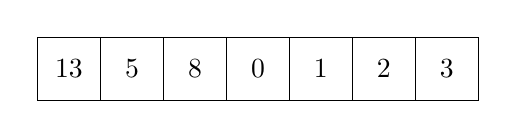
\begin{tikzpicture}
      \matrix (A) [matrix of nodes, nodes={draw, minimum size=8mm},
          column sep=-\pgflinewidth]{
          13 & 5 & 8 & 0 & 1 & 2 & 3\\};
    \end{tikzpicture}
  \end{center}
  \caption{A max heap and its array representation.}
\end{figure}

Heapsort, as you may imagine, utilizes a heap to sort elements. Heapsort
sorts its elements using two routines that 1) build a heap, 2) fix a
heap.

\begin{enumerate}
  \item \textbf{Building a heap.} The first routine is taking the array
    to sort and building a heap from it. This means ordering the array
    elements such that they obey the constraints of a max or min heap.
    For our purposes, the constructed heap will be a \emph{max heap}.
    This means that the largest element, the root of the heap, is the
    first element of the array from which the heap is built.
  \item \textbf{Fixing a heap.} The second routine is needed as we sort
    the array. The gist of Heapsort is that the largest array elements
    are repeatedly removed from the top of the heap and placed at the
    end of the sorted array, if the array is to be sorted in increasing
    order. After removing the largest element from the heap, the heap
    needs to be \emph{fixed} so that it once again obeys the constraints
    of a heap.
\end{enumerate}

In the following Python code for Heapsort, you will notice a lot of
indices are shifted down by 1. Why is this? Recall how indices of
children are computed. The formula of the left child of $k$ being $2k$
only works assuming 1-based indexing. We, in Computer Science,
especially in \textbf{C}, use 0-based indexing. So, we will run the
algorithm assuming 1-based indexing for the Heapsort algorithm itself,
subtracting 1 on each array index access to account for 0-based
indexing.

\begin{pylisting}{Heap maintenance in Python}
def max_child(A: list, first: int, last: int):
    left = 2 * first
    right = left + 1
    if right <= last and A[right - 1] > A[left - 1]:
        return right
    return left

def fix_heap(A: list, first: int, last: int):
    found = False
    mother = first
    great = max_child(A, mother, last)

    while mother <= last // 2 and not found:
        if A[mother - 1] < A[great - 1]:
            A[mother - 1], A[great - 1] = A[great - 1], A[mother - 1]
            mother = great
            great = max_child(A, mother, last)
        else:
            found = True
\end{pylisting}

\begin{pylisting}{Heapsort in Python}
def build_heap(A: list, first: int, last: int):
    for father in range(last // 2, first - 1, -1):
        fix_heap(A, father, last)

def heap_sort(A: list):
    first = 1
    last = len(A)
    build_heap(A, first, last)
    for leaf in range(last, first, -1):
        A[first - 1], A[leaf - 1] = A[leaf - 1], A[first - 1]
        fix_heap(A, first, leaf - 1)
\end{pylisting}

\section{Quicksort}

\epigraph{\emph{If debugging is the process of removing software bugs,
then programming must be the process of putting them in.}}{---Edsger
Dijkstra}

\noindent
Quicksort (sometimes called partition-exchange sort) was developed by
British computer scientist C.A.R. ``Tony'' Hoare in 1959 and published
in 1961. It is perhaps the most commonly used algorithm for sorting (by
competent programmers).  When implemented well, it is the fastest known
algorithm that sorts using \emph{comparisons}. It is usually two or
three times faster than its main competitors, Merge Sort and Heapsort.
It does, though, have a worst case performance of $O(n^2)$ while its
competitors are strictly $O(n \log n)$ in their worst case.

Quicksort is a divide-and-conquer algorithm. It partitions
arrays into two sub-arrays by selecting an element from the array and
designating it as a pivot. Elements in the array that are less than the
pivot go to the left sub-array, and elements in the array that are
greater than or equal to the pivot go to the right sub-array.

Note that Quicksort is an \emph{in-place} algorithm, meaning it doesn't
allocate additional memory for sub-arrays to hold partitioned elements.
Instead, Quicksort utilizes a subroutine called \texttt{partition()}
that places elements less than the pivot into the left side of the array
and elements greater than or equal to the pivot into the right side and
returns the index that indicates the division between the partitioned
parts of the array. Quicksort is then applied recursively on the
partitioned parts of the array, thereby sorting each array partition
containing at least one element. Like with the Heapsort algorithm, the
provided Quicksort pseudocode operates on 1-based indexing, subtracting
one to account for 0-based indexing whenever array elements are
accessed.

\begin{pylisting}{Partition in Python}
def partition(A: list, lo: int, hi: int):
    i = lo - 1
    for j in range(lo, hi):
        if A[j - 1] < A[hi - 1]:
            i += 1
            A[i - 1], A[j - 1] = A[j - 1], A[i - 1]
    A[i], A[hi - 1] = A[hi - 1], A[i]
    return i + 1
\end{pylisting}

\begin{pylisting}{Recursive Quicksort in Python}
# A recursive helper function for Quicksort.
def quick_sorter(A: list, lo: int, hi: int):
    if lo < hi:
        p = partition(A, lo, hi)
        quick_sorter(A, lo, p - 1)
        quick_sorter(A, p + 1, hi)

def quick_sort(A: list):
    quick_sorter(A, 1, len(A))
\end{pylisting}

\input{sections/batcher.tex}
\section{Your Task}

As stated previously, your task for this assignment is to write a shell script,
or more specifically, a \Bash{} script. You will use this script to
produce plots of a provided \C{} program. The provided program can be
found in the resources repository.

All the program does is print the Collatz sequence starting from some positive
integer $n$. For those unacquainted with Collatz sequences, or more broadly, the
\emph{Collatz conjecture}, the setup is as follows: We will create a sequence of
integers $S$ starting with some positive integer $n$. That is, $S_1 = n$. The
next term of the sequence is based on the previous term of the sequence. In this
case, $S_2$, the second term of the sequence, is based on $S_1$, the first term
of the sequence. For any $S_{k+1}$ where $k > 0$, the following relation holds:
$$
\begin{aligned}
S_{k+1} =
  \begin{cases}
    1+3S_k  &\text{if $S_k$ is odd} \\
    \frac{1}{2}S_k &\text{if $S_k$ is even}
  \end{cases}
\end{aligned}
$$
The conjecture itself is that any sequence following this relation always ends
with the last term being $1$, no matter what $n$ was used to start the sequence
with. This has never been proved. If you do find a sequence that does not terminate, then you \emph{may be famous}, but more likely \emph{your code has a bug}.
According to Paul Erd\H{o}s, ``Mathematics may
not be ready for such problems.''

Using the provided Collatz program, you are expected to:
\begin{enumerate}
  \item Familiarize yourself with the syntax of \C{}.
  \item Understand what the provided program is doing. You will want to attend
    section for any parts you are unsure about.
  \item Produce interesting plots using the Collatz sequences produced by the
    provided program. You should use \texttt{gnuplot} to produce these plots,
    and everything should be automated by means of a \Bash{} script.
\end{enumerate}

Refer to Figures \ref{figure:collatz-length}, \ref{figure:collatz-maxval}, and
\ref{figure:collatz-hist} for example plots that were created using the provided
program. Now that you know your task, we will now give a brief overview on
\Bash{} scripting.

\begin{figure}[htb]
  \centering
  \input{figures/collatz_length.tex}
  \caption{\label{figure:collatz-length}
    The length of Collatz sequences starting from $n \in \{\,2,\dots,10000\,\}$.
  }
\end{figure}

\begin{figure}[bth]
  \centering
  \input{figures/collatz_maxval.tex}
  \caption{\label{figure:collatz-maxval}
    The maximum values for Collatz sequences starting from $n \in
    \{\,2,\dots,10000\,\}$.
  }
\end{figure}

\begin{figure}[bth]
  \centering
  \input{figures/collatz_hist.tex}
  \caption{\label{figure:collatz-hist}
    A histogram of Collatz sequence lengths starting from $n \in
    \{\,2,\dots,10000\,\}$.
  }
\end{figure}

\section{Sets}

For this assignment, you are required to use a \emph{set} to track which
command-line options are specified when your program is run. The code
for sets is given in the resources repository in \texttt{set.h}.
\textcolor{red}{You may not modify this file.} Make sure to take the
time to go through and understand the code.

For manipulating the bits in a set, we use bit-wise operators. These
operators, as the name suggests, will perform an operation on every bit
in a number. The following are the six bit-wise operators specified in
\textbf{C}:

\begin{center}
  \begin{tabular}{|c|l|l|}
    \hline
    \verb|&| & bit-wise AND & Performs the AND operation on every bit
    of two numbers. \\
    \hline
    \verb||| & bit-wise OR & Performs the OR operation on every bit of
    two numbers. \\
    \hline
    \verb|~| & bit-wise NOT & Inverts all bits in the given number. \\
    \hline
    \verb|^| & bit-wise XOR & Performs the exclusive-OR operation on
    every bit of two numbers. \\
    \hline
    \verb|<<| & left shift & Shifts bits in a number to the left by a
    specified number of bits. \\
    \hline
    \verb|>>| & right shift & Shifts bits in a number to the right by a
    specified number of bits. \\
    \hline
  \end{tabular}
\end{center}

\noindent Recall that the basic set operations are: \emph{membership},
\emph{union}, \emph{intersection} and \emph{negation}. The functions
implementing these set operations are implemented for you. Using these
functions, you will set (make the bit 1) or clear (make the bit 0) bits
in the \texttt{Set} depending on the command-line options read by
\texttt{getopt()}. You can then check the states of all the bits (the
members) of the \texttt{Set} using a single \texttt{for} loop and
execute the corresponding sort. Note: you most likely won't use all the
functions, but you \emph{must} use sets to track which command-line
options are specified when running your program.

\begin{funcdoc}{\texttt{Set empty\_set(void)}}
  This function is used to return an empty set. In this context, an empty
  set would be a set in which all bits are equal to 0.
\end{funcdoc}

\begin{funcdoc}{\texttt{bool member\_set(uint32\_t x, Set s)}}

\begin{align*}
  x \in s \iff x\, \text{is a member of set}\, s
\end{align*}

  \noindent This function returns a \texttt{bool} indicating the
  presence of the given value \texttt{x} in the set \texttt{s}. The
  bit-wise AND operator is used to determine set membership. The first
  operand for the AND operation is the set \texttt{s}. The second
  operand is the value obtained by left shifting 1 \texttt{x} number of
  times. If the result of the AND operation is a non-zero value, then
  \texttt{x} is a member of \texttt{s} and \texttt{true} is returned to
  indicate this. \texttt{false} is returned if the result of the AND
  operation is 0.
\end{funcdoc}

\begin{funcdoc}{\texttt{Set insert\_set(uint32\_t x, Set s)}}
  This function inserts \texttt{x} into \texttt{s}. That is, it returns
  set \texttt{s} with the bit corresponding to \texttt{x} set to 1.
  Here, the bit is set using the bit-wise OR operator. The first operand
  for the OR operation is the set \texttt{s}. The second operand is
  value obtained by left shifting 1 by \texttt{x} number of bits.
\end{funcdoc}

\begin{funcdoc}{\texttt{Set delete\_set(uint32\_t x, Set s)}}

\begin{align*}
  s - x = \{y | y \in s \land y \ne x\}
\end{align*}

  This function deletes (removes) \texttt{x} from \texttt{s}. That is,
  it returns set \texttt{s} with the bit corresponding to \texttt{x}
  cleared to 0. Here, the bit is cleared using the bit-wise AND
  operator. The first operand for the AND operation is the set
  \texttt{s}. The second operand is a negation of the number 1 left
  shifted to the same position that \texttt{x} would occupy in the set.
  This means that the bits of the second operand are all 1s except for
  the bit at \texttt{x}'s position. The function returns set \texttt{s}
  after removing \texttt{x}.
\end{funcdoc}

\begin{funcdoc}{\texttt{Set union\_set(Set s, Set t)}}

\begin{align*}
  s \cup t = \{x | x \in s \lor x \in  t\}
\end{align*}

  \noindent The union of two sets is a collection of all elements in
  both sets. Here, to calculate the union of the two sets \texttt{s} and
  \texttt{t}, we need to use the OR operator. Only the bits
  corresponding to members that are equal to 1 in either \texttt{s} or
  \texttt{t} are in the new set returned by the function.
\end{funcdoc}

\begin{funcdoc}{\texttt{Set intersect\_set(Set s, Set t)}}

\begin{align*}
  s \cap t = \{x | x \in s \land x \in  t\}
\end{align*}

  \noindent The intersection of two sets is a collection of elements that
  are common to both sets. Here, to calculate the intersection of the
  two sets \texttt{s} and \texttt{t}, we need to use the AND operator.
  Only the bits corresponding to members that are equal to 1 in both
  \texttt{s} and \texttt{t} are in the new set returned by the function.
\end{funcdoc}

\begin{funcdoc}{\texttt{Set difference\_set(Set s, Set t)}}
  The difference of two sets refers to the elements of set \texttt{s}
  which are not in set \texttt{t}. In other words, it refers to the
  members of set \texttt{s} that are unique to set \texttt{s}. The
  difference is calculated using the AND operator where the two operands
  are set \texttt{s} and the negation of set \texttt{t}. The function
  then returns the set of elements in \texttt{s} that are not in
  \texttt{t}.

  This function can be used to find the complement of a given set as well,
  in which case the first operand would be the universal set $\mathbb{U}$
  and the second operand would be the set you want to complement as shown
  below.
\end{funcdoc}

\begin{align*}
  \overline{s} = \{ x | x \notin s\} = \mathbb{U} -s
\end{align*}

\begin{funcdoc}{\texttt{Set complement\_set(Set s)}}
  This function is used to return the complement of a given set. By
  complement we mean that all bits in the set are flipped using the NOT
  operator. Thus, the set that is returned contains all the elements of
  the universal set $\mathbb{U}$ that are not in \texttt{s} and contains
  none of the elements that are present in \texttt{s}.
\end{funcdoc}

\section{Testing}

\begin{itemize}
  \item You will test each of the sorts specified by command-line option
    by sorting an array of pseudorandom numbers generated with
    \texttt{random()}. Each of your sorts should sort the \emph{same}
    pseudorandom array. \textcolor{red}{Hint: make use of
    \texttt{srandom()}.}
  \item The pseudorandom numbers generated by \texttt{random()} should
    be \emph{bit-masked} to fit in \emph{30} bits. \textcolor{red}{Hint: use
    bit-wise AND.}
  \item Your test harness \emph{must} be able to test your sorts with
    array sizes \emph{up to the memory limit of the computer}. That
    means that you will need to dynamically allocate the array.
  \item Your program should have no \emph{memory leaks}. Make sure you
    \texttt{free()} before exiting. \texttt{valgrind} should pass
    cleanly with any combination of the specified command-line options.
  \item Your algorithms \emph{must} correctly sort. Any algorithm that
    does not sort correctly will receive a \emph{zero}.
\end{itemize}

A large part of this assignment is understanding and comparing the
performance of various sorting algorithms. You essentially conducting an
experiment. As stated in \S\ref{task}, you \emph{must} collect the following
statistics on each algorithm:

\begin{itemize}
  \item The \emph{size} of the array,
  \item The number of \emph{moves} required (each time you transfer an
    element in the array, that counts), and
  \item The number of \emph{comparisons} required (comparisons
    \emph{only} count for \emph{elements}, not for logic).
\end{itemize}

\section{Output}
\epigraph{\emph{Books are not made to be believed, but to be subjected to inquiry. When we consider a book, we mustn’t ask ourselves what it says but what it means.}}{---Umberto Eco}

\noindent
The output your test harness produces \emph{must} be formatted like in
the following examples:

\begin{shlisting}{}
$ ./sorting -q -n 1000 -p 0
Quick Sort, 1000 elements, 18642 moves, 10531 compares
$ ./sorting -h -n 15 -p 0
Heap Sort, 15 elements, 144 moves, 70 compares
$ ./sorting -a -n 15
Shell Sort, 15 elements, 90 moves, 59 compares
     34732749     42067670     54998264    102476060    104268822
    134750049    182960600    538219612    629948093    783585680
    954916333    966879077    989854347    994582085   1072766566
Batcher Sort, 15 elements, 90 moves, 59 compares
     34732749     42067670     54998264    102476060    104268822
    134750049    182960600    538219612    629948093    783585680
    954916333    966879077    989854347    994582085   1072766566
Heap Sort, 15 elements, 144 moves, 70 compares
     34732749     42067670     54998264    102476060    104268822
    134750049    182960600    538219612    629948093    783585680
    954916333    966879077    989854347    994582085   1072766566
Quick Sort, 15 elements, 135 moves, 51 compares
     34732749     42067670     54998264    102476060    104268822
    134750049    182960600    538219612    629948093    783585680
    954916333    966879077    989854347    994582085   1072766566
\end{shlisting}

For each sort that was specified, print its name, the statistics for the
run, then the specified number of array elements to print. The array
elements should be printed out in a table with 5 columns. Each array
element should be printed with a width of 13. You should make use of the
following \texttt{printf()} statement:

\begin{clisting}{}
printf("%13" PRIu32); // Include <inttypes.h> for PRIu32.
\end{clisting}

\section{Statistics}
\epigraph{\emph{There are three types of lies---lies, damn lies, and statistics.}}{%
---Benjamin Disraeli}

\noindent
To facilitate the gathering of statistics, you will be given,
\textcolor{red}{\emph{and must use}}, a small statistics module. The
module itself revolves around the following struct:

\begin{clisting}{}
typedef struct {
  uint64_t moves;
  uint64_t comparisons;
} Stats;
\end{clisting}

The module also includes functions to \emph{compare}, \emph{swap}, and
\emph{move} elements.

\begin{funcdoc}{int cmp(Stats *stats, uint32\_t x, uint32\_t y)}
  Compares \texttt{x} and \texttt{y} and increments the
  \texttt{comparisons} field in \texttt{stats}. Returns \texttt{-1} if
  \texttt{x} is less than \texttt{y}, \texttt{0} if \texttt{x} is equal
  to \texttt{y}, and \texttt{1} if \texttt{x} is greater than
  \texttt{y}.
\end{funcdoc}

\begin{funcdoc}{uint32\_t move(Stats *stats, uint32\_t x)}
  ``Moves'' \texttt{x} by incrementing the \texttt{moves} field in
  \texttt{stats} and returning \texttt{x}. This is intended for use in
  Insertion Sort and Shell Sort, where array elements aren't swapped,
  but instead moved and stored in a temporary variable.
\end{funcdoc}

\begin{funcdoc}{void swap(Stats *stats, uint32\_t *x, uint32\_t *y)}
  Swaps the elements pointed to by pointers \texttt{x} and \texttt{y},
  incrementing the \texttt{moves} field in \texttt{stats} by 3 to
  reflect a swap using a temporary variable.
\end{funcdoc}

\begin{funcdoc}{void reset(Stats *stats)}
  Resets \texttt{stats}, setting the \texttt{moves} field and
  \texttt{comparisons} field to 0. It is possible that you don't end up
  using this specific function, depending on your usage of the
  \texttt{Stats} \texttt{struct}.
\end{funcdoc}

\section{Deliverables}

\noindent You will need to turn in the following source code and header files:

\begin{enumerate}
  \item \texttt{bf.h}: Defines the interface for the Bloom filter ADT.
    \textcolor{red}{Do not modify this.}

  \item \texttt{bf.c}: Contains the implementation of the Bloom filter
    ADT.

  \item \texttt{bv.h}: Defines the interface for the bit vector ADT.
    \textcolor{red}{Do not modify this.}

  \item \texttt{bv.c}: Contains the implementation of the bit vector
    ADT.

  \item \texttt{ht.h}: Defines the interface for the hash table ADT and the hash
    table iterator ADT. \textcolor{red}{Do not modify this.}

  \item \texttt{ht.c}: Contains the implementation of the hash table
    ADT and the hash table iterator ADT.

  \item \texttt{identify.c}: Contains \texttt{main()} and the implementation of
    the author identification program.

  \item \texttt{metric.h}: Defines the enumeration for the distance metrics and
    their respective names stored in an array of strings. \textcolor{red}{Do not
    modify this.}

  \item \texttt{node.h}: Defines the interface for the node ADT.
    \textcolor{red}{Do not modify this.}

  \item \texttt{node.c}: Contains the implementation of the node ADT.

  \item \texttt{parser.h}: Defines the interface for the regex parsing
    module. \textcolor{red}{Do not modify this.}

  \item \texttt{parser.c}: Contains the implementation of the regex
    parsing module.

  \item \texttt{pq.h}: Defines the interface for the priority queue ADT.
    \textcolor{red}{Do not modify this.}

  \item \texttt{pq.c}: Contains the implementation for the priority queue ADT.

  \item \texttt{salts.h}: Defines the primary, secondary, and tertiary
    salts to be used in your Bloom filter implementation. Also defines
    the salt used by the hash table in your hash table implementation.

  \item \texttt{speck.h}: Defines the interface for the hash function
    using the SPECK cipher. \textcolor{red}{Do not modify this.}

  \item \texttt{speck.c}: Contains the implementation of the hash
    function using the SPECK cipher. \textcolor{red}{Do not modify this.}

  \item \texttt{text.h}: Defines the interface for the text ADT.
    \textcolor{red}{Do not modify this.}

  \item \texttt{text.c}: Contains the implementation for the text ADT.
\end{enumerate}

You may have other source and header files, but \emph{do not try to be
overly clever}. You will also need to turn in the following:

\begin{enumerate}
  \item \texttt{Makefile}: This is a file that will allow the grader to
    type \texttt{make} to compile your program.

    \begin{itemize}
      \item \texttt{CC = clang} must be specified.
      \item \texttt{CFLAGS = -Wall -Wextra -Werror -Wpedantic}
        must be included.
      \item \texttt{make} should build the \texttt{identify}
        executable, as should \texttt{make all} and \texttt{make
        identify}.
      \item \texttt{make clean} must remove all files that are compiler
        generated.
      \item \texttt{make format} should format all your source code,
        including the header files.
    \end{itemize}

  \item Your code must pass \texttt{scan-build} \emph{cleanly}. If there
    are any bugs or errors that are false positives, document them and
    explain why they are false positives in your \texttt{README.md}.

  \item \texttt{README.md}: This must be in \emph{Markdown}. This must
    describe how to use your program and \texttt{Makefile}. This
    includes listing and explaining the command-line options that your
    program accepts. Any false positives reported by \texttt{scan-build}
    should go here as well.

  \item \texttt{DESIGN.pdf}: This \emph{must} be a PDF. The design
    document should describe your design for your program with enough
    detail that a sufficiently knowledgeable programmer would be able to
    replicate your implementation. This does not mean copying your
    entire program in verbatim. You should instead describe how your
    program works with supporting pseudocode. For this program, pay
    extra attention to how you build each necessary component.

  \item \texttt{WRITEUP.pdf}: This document \emph{must} be a PDF. The
    writeup must discuss what you observe about your program's behavior as you
    tune the number of noise words that are filtered out and the amount of text
    that you feed your program. Does your program accurately identify the author
    for a small passage of text? What about a large passage of text? How do the
    different metrics (Euclidean, Manhattan, Cosine) compare against each other?
\end{enumerate}

\section{Submission}

Refer back assignment 0 for the instructions on how to properly submit your
assignment through \texttt{git}. Remember: \emph{add}, \emph{commit}, and
\emph{push}!

\textcolor{red}{Your assignment is turned in \emph{only} after you have pushed
and submitted the commit ID you want graded on Canvas. ``I forgot to push'' and
``I forgot to submit my commit ID'' are not valid excuses. It is \emph{highly}
recommended to commit and push your changes \emph{often}.}

\section{Supplemental Readings}

\epigraph{\emph{It is good that Pol Pot is dead. I feel no sorrow.\ldots
I hope he suffers after death.}}{---Ta Mok}

\noindent
\begin{itemize}
  \item \textit{The C Programming Language} by Kernighan \& Ritchie
  \begin{itemize}
    \item Chapter 5 \S 5.7
    \item Chapter 7
  \end{itemize}
  \item \textit{Introduction to Algorithms} by T.\ Cormen, C.\
    Leiserson, R.\ Rivest, \& C.\ Stein
    \begin{itemize}
      \item Chapter 11 (Hash tables and hash functions)
      \item Chapter 12 (Binary Search Trees)
    \end{itemize}
  \item \textit{Introduction to the Theory of Computation} by M.\ Sipser
    \begin{itemize}
      \item Chapter 1 \S 1.3 (Regular expressions)
    \end{itemize}
\end{itemize}


\monkey{Code Monkey like Fritos \\
Code Monkey like Tab and Mountain Dew \\
Code Monkey very simple man \\
With big warm fuzzy secret heart: \\
Code Monkey like you}

\end{document}
